\hypertarget{a00010}{
\section{Dokumentacja klasy ASS8.Klient.klientOdpDownload}
\label{d7/dec/a00010}\index{ASS8::Klient::klientOdpDownload@{ASS8::Klient::klientOdpDownload}}
}
Klasa zawiera dane do serializacji odpowiedzi o ściągnięcie pliku.  


Dziedziczy \hyperlink{a00007}{ASS8::Klient::klientBase}.

Diagram współpracy dla ASS8.Klient.klientOdpDownload:\nopagebreak
\begin{figure}[H]
\begin{center}
\leavevmode
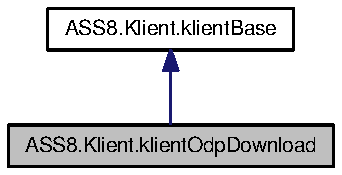
\includegraphics[width=200pt]{d3/d2a/a00195}
\end{center}
\end{figure}
\subsection*{Metody publiczne}
\begin{CompactItemize}
\item 
\hyperlink{a00010_39b02a7d62f5f5d1fc3f027bc1ab666b}{klientOdpDownload} ()
\item 
\hyperlink{a00010_31174bd92b052586e1bb093bf631f330}{klientOdpDownload} (int id, int oper, string act)
\end{CompactItemize}
\subsection*{Właściwości}
\begin{CompactItemize}
\item 
string \hyperlink{a00010_f1e41ed2ca8b161225883d79faa35121}{action}\hspace{0.3cm}{\tt  \mbox{[}get, set\mbox{]}}
\end{CompactItemize}
\subsection*{Atrybuty prywatne}
\begin{CompactItemize}
\item 
string \hyperlink{a00010_50dcb80ebd84c9929250c659e169fea9}{pAction}
\end{CompactItemize}


\subsection{Opis szczegółowy}
Klasa zawiera dane do serializacji odpowiedzi o ściągnięcie pliku. 



Definicja w linii 253 pliku XmlRequestsClass.cs.

\subsection{Dokumentacja konstruktora i destruktora}
\hypertarget{a00010_39b02a7d62f5f5d1fc3f027bc1ab666b}{
\index{ASS8::Klient::klientOdpDownload@{ASS8::Klient::klientOdpDownload}!klientOdpDownload@{klientOdpDownload}}
\index{klientOdpDownload@{klientOdpDownload}!ASS8::Klient::klientOdpDownload@{ASS8::Klient::klientOdpDownload}}
\subsubsection[{klientOdpDownload}]{\setlength{\rightskip}{0pt plus 5cm}ASS8.Klient.klientOdpDownload.klientOdpDownload ()}}
\label{d7/dec/a00010_39b02a7d62f5f5d1fc3f027bc1ab666b}




Definicja w linii 256 pliku XmlRequestsClass.cs.\hypertarget{a00010_31174bd92b052586e1bb093bf631f330}{
\index{ASS8::Klient::klientOdpDownload@{ASS8::Klient::klientOdpDownload}!klientOdpDownload@{klientOdpDownload}}
\index{klientOdpDownload@{klientOdpDownload}!ASS8::Klient::klientOdpDownload@{ASS8::Klient::klientOdpDownload}}
\subsubsection[{klientOdpDownload}]{\setlength{\rightskip}{0pt plus 5cm}ASS8.Klient.klientOdpDownload.klientOdpDownload (int {\em id}, \/  int {\em oper}, \/  string {\em act})}}
\label{d7/dec/a00010_31174bd92b052586e1bb093bf631f330}




Definicja w linii 257 pliku XmlRequestsClass.cs.

\subsection{Dokumentacja atrybutów składowych}
\hypertarget{a00010_50dcb80ebd84c9929250c659e169fea9}{
\index{ASS8::Klient::klientOdpDownload@{ASS8::Klient::klientOdpDownload}!pAction@{pAction}}
\index{pAction@{pAction}!ASS8::Klient::klientOdpDownload@{ASS8::Klient::klientOdpDownload}}
\subsubsection[{pAction}]{\setlength{\rightskip}{0pt plus 5cm}string {\bf ASS8.Klient.klientOdpDownload.pAction}\hspace{0.3cm}{\tt  \mbox{[}private\mbox{]}}}}
\label{d7/dec/a00010_50dcb80ebd84c9929250c659e169fea9}




Definicja w linii 255 pliku XmlRequestsClass.cs.

\subsection{Dokumentacja właściwości}
\hypertarget{a00010_f1e41ed2ca8b161225883d79faa35121}{
\index{ASS8::Klient::klientOdpDownload@{ASS8::Klient::klientOdpDownload}!action@{action}}
\index{action@{action}!ASS8::Klient::klientOdpDownload@{ASS8::Klient::klientOdpDownload}}
\subsubsection[{action}]{\setlength{\rightskip}{0pt plus 5cm}string ASS8.Klient.klientOdpDownload.action\hspace{0.3cm}{\tt  \mbox{[}get, set\mbox{]}}}}
\label{d7/dec/a00010_f1e41ed2ca8b161225883d79faa35121}




Definicja w linii 264 pliku XmlRequestsClass.cs.

Dokumentacja dla tej klasy została wygenerowana z pliku:\begin{CompactItemize}
\item 
\hyperlink{a00055}{XmlRequestsClass.cs}\end{CompactItemize}
